\documentclass[journal]{IEEEtran}
\usepackage[hyphens]{url}
\begin{document}
\title{Twitter as an Alternative Review Site}

\author{Sin\'ead~Dickson
\thanks{Sin\'ead Dickson was with the School of Computer Science and Statistics, the University of Dublin, Trinity College, Dublin, Ireland (e-mail: sdickson@tcd.ie).}
\thanks{Manuscript received April 2019.}}

\maketitle

\begin{abstract}
The increasing amount of information available on the internet means that recommender systems are growing in importance. Recommender systems help users to overcome information overload. They aim to help users to quickly find information relevant to them.

Online reviews are an important source of consumer opinions. They provide large quantities of data on consumer preferences and opinions. Twitter is a widely used microblogging social media platform, with 126 million daily users and 500 million tweets posted per day. Tweets posted to the site can often take the form of a review. This project will focus on harnessing these reviews and using them to help generate recommendations in the CoRE recommender system.

This paper proposes a method of first extracting review-like tweets from Twitter and then incorporating the sentiment of those tweets into a recommender system. This research aims to evaluate to what extent Twitter can provide a suitable source of online reviews that can be used effectively in the generation of recommendations in a recommender system. The project focused on reviews about hotels in Dublin.

This research explores the use of various classification algorithms and feature representations to classify whether tweets contain reviews. The sentiment of these review-like tweets is calculated and used to re-rank the CoRE recommender system.

The classification results were promising, showing that text classification is a valid method of extracting tweets from reviews. The best performing classifier was the Support Vector Machine. It achieved a precision score of 74\%, a recall score of 74\%, an f1-score of 73\% and an accuracy score of 74.4\%.

Incorporating the sentiment score into the CoRE had the desired effect and adjusted the rankings of the hotels. However, in terms of mean percentile rank (MPR) SentiCoRE performed worse that CoRE. 
\end{abstract}

\begin{IEEEkeywords}
Twitter, Review, Recommender Systems, Machine~Learning, Classification.
\end{IEEEkeywords}

\section{Introduction}
\IEEEPARstart{T}{he rapid} development and expansion of the internet has introduced new ways for individuals to express their opinions and disseminate their views. Online reviews have become a hugely important source of information for consumers. They play an important role in determining whether a person is satisfied with a product or service. Online reviews provide a huge amount of data on consumer preferences. 

This paper will focus on Twitter, a microblogging social media site, where users can post short blocks of text of no more than 280 characters. Twitter currently has ~126 million people who use the site daily, with over 500 million tweets posted per day \cite{Twitter2019}. These tweets can often take the form of a review and can give insight into consumers' opinions on the entities with which they interact. With millions of tweets being posted every day, Twitter has a huge potential source of underutilised reviews.

Traditional online review sites include websites like TripAdvisor, Foursquare and Yelp. Often these sites have a dedicated area for feedback and encourage users to leave reviews of their hotels, restaurants or products. In our opinion, this method of obtaining reviews can sometimes result in more forced, manufactured, less reliable reviews. It is our contention that users tend to post their genuine feelings more spontaneously and frequently to Twitter. Users often wouldn't consider their posts to be a 'review' in the formal sense of the word and not in the same way they would consider a review left in the dedicated feedback area of another website.

In this paper, we will investigate to what extent Twitter can provide a suitable source of online reviews that can be used effectively in the generation of recommendations in a recommender system. We will explore methods of classifying review-like tweets, identifying the sentiment of the reviews and the effect of using this data in a recommender system. The project will focus on tweets that mention or discuss hotels in the Dublin area.

Twitter data has a different format to standard long-form text and needs to be treated differently. Tweets are short with a maximum of 280 characters, which has led to the use of particular characteristic features. Tweets are generally very informal, using casual language and slang. They contain features like hashtags, emojis, Twitter handles, URLs, images, videos and gifs, which don't occur in standard text. The short length and non-standard features can create a challenge for standard text classification algorithms and standard machine learning feature representations. 

This paper is organised as follows: Section II presents a review of the literature relating to this project. Section III describes the design and methodology of the project. It outlines how the data was collected, filtered, processed, and annotated. It also describes the classification techniques used, the sentiment analysis tool used and how the sentiment scores produced were applied to the recommender system CoRE \cite{core2019}. Section IV presents an evaluation and discussion of the results of this research. Finally, Section V gives our conclusions and future works.
\section{Related Works}

Classification is the process of mapping observations into classes, based on some set of training data. A number of papers have investigated the performance of classification algorithms applied to Twitter data. \cite{Berm2010} investigated the performance of Support Vector Machines (SVM) and Multinomial Naïve Bayes (MNB) in classifying the sentiment of short versus long form text documents. MNB achieved better accuracy than SVM on the short form documents, from both Twitter and Blippr (a micro-review site). \cite{Rane2018} also examined the performance of classification algorithms applied to Twitter data, specifically reviews about US Airline Services. Doc2Vec feature representation was used, which involves mapping each document to a vector in space. In this study, each paragraph was mapped to a vector. They found the Random Forest Classifier performed the best.

\cite{sriram2010} evaluated the performance of different feature representations for classifying tweets into a set of generic classes: News, Opinions, Events, Deals and Private Messages. They proposed an eight-feature technique. Eight features were extracted from the tweets, one nominal (author) and seven binary (whether the tweet contained shortened words/slang, time-event phrases, opinion words, emphasis on words, currency or percentage signs, the username at the start, the username mid-tweet). They compared this technique to bag-of-words and found it performed significantly better. \cite{Berm2010} also experimented with different feature representations for Twitter data. They found that extending the unigram feature representation did not improve classification accuracy but extracting Part-of-Speech features and punctuation did. 

An Ensemble Classifier (EC) was proposed by \cite{Ankit2018} to classify the sentiment of tweets. The proposed weighted EC outperforms each of the individual base classifiers, as well as the majority voting EC. \cite{Kanakaraj2015} also found that ECs performed better in classifying the sentiment of tweets than base classifiers. They compared several base classifiers and ECs, and found the ensemble methods outperformed the individual base classifiers, with Extremely Randomised Trees performing the best.

Sentiment analysis is the process of identifying the opinion expressed about a particular subject in some text. The aim is to determine whether the opinion is positive, negative or neutral, and to what extent. The two main approaches to sentiment analysis are: lexicon based approaches and supervised machine learning based approaches. A lexicon-based approach works by classifying a sentence based on the number of opinion words (positive or negative words) in the sentence. Supervised machine learning approaches require labelled training data to learn a function that maps an input to an output.

\cite{Bhuta2014} reviewed different methods for the sentiment analysis of Twitter data. These included a lexicon approach and three supervised learning methods, Naive Bayes, Maximum Entropy and SVM. The three supervised learning methods outperformed the lexicon-based approach. The disadvantage of the supervised machine learning approaches is that it can be hard to know exactly what is having an effect on the algorithm and how to improve it.

The Stanford NLP Group's Sentiment Analyser \cite{stanfordSentiment2013} introduced a Recursive Neural Tensor Network (RNTN) and Sentiment Treebank. The Sentiment Treebank extended the corpus of movie reviews originally collected by Pang and Lee \cite{panglee2004}. The sentences were relabelled at a phrase level, producing a labelled parse-tree for each review. The Treebank has more finely grained sentiment labels than the original corpus, which improved how the compositional effects of sentiment in language were captured. The Sentiment Analyser achieved accuracy of 85.4\% in single sentence positive/negative classification.

Recommender systems provide suggestions for items that are most likely to be of interest to a particular user \cite{Ricci2015}. The two main methods that recommender systems use to generate recommendations are: Collaborative Filtering methods and Content-Based recommender methods. Collaborative Filtering methods analyse the behaviour of a collection of users and use this information to make recommendations based upon what users similar to the current user have liked. Content-Based (CB) recommender methods use the descriptive features of items and the preferences of individual users. CB methods recommend items similar to items the user liked or purchased in the past. Recommender systems often incorporate context information in an attempt to provide more personalised reviews. Context-aware recommender systems use contextual information (time, location, company, etc.) to improve their recommendations. The concept is that the same user could prefer different items under different conditions.

A number of hotel recommender systems have been proposed in previous literature. \cite{levi2012} proposed a cold start, context-based hotel recommender system, which uses the text of online reviews from Tripadvisor and Venere as its main data. The system asks the user to identify their trip intent (business, family, etc), nationality and preferences for certain hotel features (location, service, food, etc). Hotels are recommended based on the sentiment of reviews of users who have similar context information. The sentiment score is calculated with a lexicon based approach. They reported that users were 20\% more satisfied with their recommendations. This is a promising result for this research. The hope is that incorporating review-like tweets into the CoRE recommender will also increase user satisfaction. \cite{lin2015} also uses hotel reviews collected from TripAdvisor to recommend hotels. The system tracks the user's gestures on a mobile device to identify what part of the review the user has focused on or 'seriously read'. Feature extraction is used to extract the aspects of hotels (e.g room, food, price etc) the user considers important, and build a user interest profile. Hotels are recommended based on the user profile. The score is calculated based on the sentiment of the reviews about the aspects of the hotels the user prefers.
\section{Design and Methodology}

\subsection{Data Collection}
The data was collected using the Twitter Streaming API \footnote{\url{https://developer.twitter.com}} between October 2017 and September 2018. The Streaming API allows you to stream real-time tweets. A location filter was specified so that only tweets posted from within the bounding box of Dublin were returned (Figure ~\ref{fig:dublinBB}). A total of 2.5 million tweets were collected.

After inspecting the collection of tweets it was found that although a bounding box had been specified, not all tweets in the collection had been posted from Dublin. A significant amount of tweets had slipped through Twitter's location filter. This meant that the first step required was to filter the dataset to ensure, as much as was possible, that all tweets related to Dublin.

\subsection{Data Filtering}
The raw dataset was cleaned and filtered, so that it only contained English language tweets posted from Dublin, and secondly so that it only contained tweets mentioning hotels.

\subsubsection{Filtering Out Non-Dublin Tweets}
All of the tweets in the dataset were Geo-tagged because they were collected with Twitter's location filter. This meant they all had location data: a specified location from which the tweet was posted. There are two types of Geo-tagged tweets, tweets with a 'Point Coordinate', a specific latitude/longitude or point coordinate, and tweets with a 'Twitter Place', a specified bounding box defining a certain place.

Only 7.23\% of the tweets in the collection had point coordinates so a combination of the Twitter place and the point coordinates was used to filter out any non-Dublin tweets that had ended up in the dataset. A bounding box for the Dublin area was defined (North Latitude: 53.425210, South Latitude: 53.223430, East Longitude: -6.043924, West Longitude: -6.447485). Tweets with a point coordinate and tweets with only a Twitter place were filtered differently. Each tweet with a point coordinate was checked to see if the point coordinate fell within the defined bounding box for Dublin. If it lay inside the box it was kept, otherwise, it was filtered out. Each tweet with a Twitter place has a bounding box specifying the location of the place. The centroid of this bounding box was calculated for each tweet. Then the centroid was checked to see if it fell within the defined bounding box for Dublin. If it lay inside the box it was kept, otherwise, it was filtered out. 

The filtered dataset consisted of 1.6 million tweets posted from Dublin between October 2017 and September 2018.

\subsubsection{Filtering Tweets About Hotels}
A list of the hotels in Dublin was compiled. This included the hotel's name and the hotel's Twitter handles (@hotelname). This list consisted of 159 hotels and Twitter handles.

The tweets were stored in a Lucene index. A fuzzy search query was used to match the tweets against each of the hotel names and hotel Twitter handles. The fuzzy search query uses a similarity measure that is based on the Damerau-Levenshtein algorithm. The maximum edits option was set to two, meaning that strings with a maximum difference of two characters would still match. This accounted for misspellings and broadened our search slightly. We experimented with higher numbers of maximum edits but found that too many irrelevant tweets were returned.

No NLP (natural language processing) technique that attempts to identify all mentions will be 100\% accurate. Users will refer to hotels in all manner of ways, anaphora like 'the hotel'. We have tried to be reasonably conservative and ensure we have a pretty clean dataset, but there are a range of ways to identify hotels that could be experimented with. 

This further filtered dataset consisted of 3115 tweets that mention hotels posted from Dublin between October 2017 and September 2018.

\subsection{Dataset Annotation}

In order to train a classifier to categorise tweets as review-like tweets, as tweets that contain some content and as irrelevant tweets, a set of tweets had to first be manually annotated. The set of 3115 tweets about hotels in Dublin was annotated. This involved building an annotation webpage where users could view tweets and assign them labels.

A simple webpage was created in order to annotate the tweets (Figure ~\ref{fig:webpage}). 

\begin{figure}[h!]
\centering
\fbox{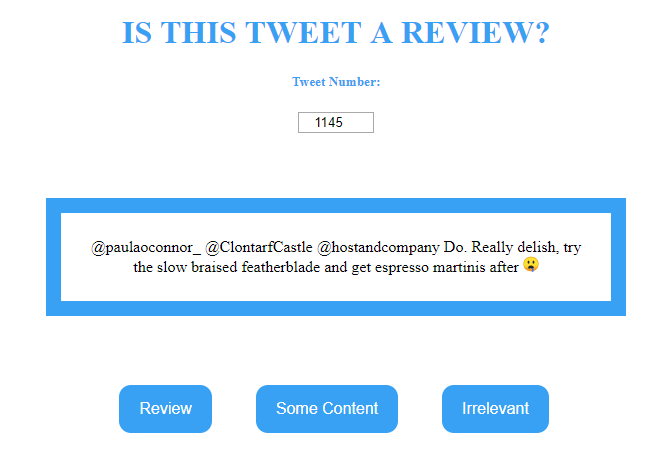
\includegraphics[width=0.95\columnwidth]{design_and_methodology/webpage.PNG}}
\caption{\label{fig:webpage} Tweet Annotation Webpage.}
\end{figure}

The text of each tweet was displayed alongside three buttons: 'Review', 'Some Content' and 'Irrelevant'. The participant could click on the option that they thought best described the tweet shown. Once they chose a label, the next tweet would be displayed. 

The following instructions, describing what a 'Review', 'Some Content' and 'Irrelevant' tweet should look like accompanied the webpage:
\begin{itemize}
    \item Review: The tweet could be considered as a review (of any aspects related to a hotel such as the venue, food, view, swimming pool, etc.) for any hotel. Examples would include: \emph{"Amazing view of the Aviva Stadium from my hotel balcony at hotel X"} (positive review), "Room service was awful at hotel Y" (negative review), \emph{"Thank you hotel X for a lovely stay"} (positive review) or \emph{"Had an awful night at hotel Y"} (negative review).
    \item Some Content: The tweet doesn't look like a review, but it does provide some information related to a hotel, such as the hotel hosts events, information on the menu, information related to accommodation, etc. Examples would include: \emph{"Hotel Z serves Tuna salad on Wednesday”} or \emph{“A packed room for the 2018 fashion conference at Hotel X”}.
    \item Irrelevant: This tweet is completely irrelevant. While perhaps mentioning the name of a hotel, the tweet doesn't give any additional information about that hotel or offer any opinions related to the hotel.
\end{itemize}

In this research, we decided to focus solely on the text of the tweets. For this reason, all images, videos and URLs were stripped from the tweets before being displayed on the annotation webpage. Images, videos and URLs could all carry valuable information and could be considered in future research. 

The annotation webpage was circulated to friends, family and members of the Adapt Research Centre to gather annotations.

\subsection{Tweet Classification}
The annotated set of tweets was used to train a series of different classifiers with different feature representations to determine which combination was most suited to the task. These classifiers were implemented using Python's Scikit Learn library \cite{scikit-learn}. The data was split into a training set and a testing set. The data was split 80:20 where 80\% was used for training and 20\% was used for testing.

\subsubsection{Data Pre-processing}

The following steps were taken to pre-process the tweets before they were used to train the classifiers:
\begin{itemize}
    \item Emojis: Emojis were removed and replaced with text using Python's Emoji library \cite{emoji}.
    \item Punctuation: The majority of special characters and punctuation was removed from the tweets. This included everything except the digits 0 - 9, the letters a - z (in upper and lower case), and the following set of symbols: . , ? ! ( ) \& ' - . 
    \item Single Characters: All single characters were removed.
    \item Case Change: Words were split on case changes. For example \emph{'MerrionHotel'} --> \emph{'Merrion Hotel'}.
    \item Word-digit Boundaries: Words were split on word-digit boundaries. For example \emph{'HouseDublin2'} --> \emph{'House Dublin 2'}.
    \item Lowercase: All text was converted to lower case.
    \item Stemming: Stemming was performed using the Word Net Lemmatizer from the Natural Language Toolkit \footnote{\url{https://www.nltk.org/}}.
    \item Stop Words: Stop words were removed in some cases using Scikit Learn's Engligh stop word list. It will be clearly stated in all cases where stop words were removed.
\end{itemize}

\subsubsection{Feature Representation}

We experimented with seven different feature extraction methods to see which performed best at classifying the Twitter data. Tweets are short with a maximum of 280 characters, which has led to the use of particular characteristic features, such as, hashtags, emojis, Twitter handles, URLs, images, videos and gifs, which don't occur in standard text. This means that standard feature extraction methods that perform well on regular, long-form text will not necessarily perform well on Twitter data.

The seven feature extraction methods implemented were:
\begin{itemize}
    \item Unigram Bag-of-Words (BOW): A unigram implementation of BOW using Scikit Learn's Count Vectorizer. In Bag-of-Words (BOW) documents are described by word occurrences. Each tweet is then represented as a feature vector consisting of ones and zeroes. One representing a term's occurrence and zero representing a term's absence.
    \item Unigram TF-IDF: A unigram implementation of TF-IDF using Scikit Learn's Count Vectorizer and TF-IDF transformer. BOW can be extended with TF-IDF (Term Frequency - Inverse Document Frequency). Term frequency is the frequency of the word in the current document. Inverse Document Frequency takes into account how often the word occurs in the whole dataset. The idea is to balance how important a term is in a document versus how important it is in the entire collection. The TF-IDF score is used to re-weight the count features produced by the Count Vectorizer.
    \item Bigram TF-IDF: A bigram implementation of TF-IDF using Scikit Learn's Count Vectorizer and TF-IDF transformer. Another extension of BOW is the use of N-grams. N-grams help to address the problem BOW has with discarding word order. An N-gram is a sequence of N consecutive terms. Combining bigrams with BOW means that occurrences of pairs of consecutive words are counted instead of individual terms.
    \item Trigram TF-IDF: A trigram implementation of TF-IDF using Scikit Learn's Count Vectorizer and TF-IDF transformer.
    \item Unigram TF-IDF (stop words removed): A unigram implementation of TF-IDF with stop words removed using Scikit Learn's Count Vectorizer, TF-IDF transformer and English stop word list.
    \item Word2Vec: Gensim's implementation of word2vec with Google's pretrained model. Word2Vec takes a dataset as its input and produces a vector space. Each word in the dataset is represented by a corresponding vector. It groups the vector of similar words together in the vector space. Cosine similarity, the cosine of the angle between two vectors, measures the similarity of vectors in the vector space.    
    \item Doc2Vec: Gensim's implementation of doc2vec, each tweet being considered a document. Doc2Vec takes the same idea as Word2Vec, but instead of words being represented by vectors, full documents are represented as vectors. This captures the relationship between words, which Word2Vec does not. Unlike Word2Vec, we built our own Doc2Vec vocabulary based on the training data.
\end{itemize}

\subsubsection{Classification Algorithms}

Thirteen different classifiers were implemented, each with their implementation from Python's Scikit Learn library \cite{scikit-learn}:
\begin{itemize}
    \item Decision Tree (DT) Classifier: DT classifiers learn simple decision rules based on the attributes of the training data. These decision rules form a tree structure which is used to predict the value of a target variable. The leaf nodes represent the class labels. When an unclassified document is received questions are asked until a leaf node is reached and the document is assigned that class.
    \item Random Forest (RF) Classifier: The RF Classifier is an ensemble classification algorithm, meaning it combines multiple base classification algorithms. It consists of multiple DT classifiers. The final class prediction is calculated by getting the average of the decisions of the individual decision trees.
    \item Multi Layer Perceptron (MLP) Classifier: The MLP Classifier is a deep, feedforward, artificial neural network. It consists of a minimum of three layers: an input layer, a hidden layer and an output layer. The input layer receives the data, the output layer makes a decision and the hidden layers approximate the function.
    \item Logistic Regression (LR) Classifier: The LR Classifier is a linear classification algorithm that uses the logistic function to model the training data. 
    \item Support Vector Machine (SVM) Classifier: The SVM Classifier is a discriminative classifier. It finds the optimum hyperplane that separates the data into the labelled classes. It aims to maximise the distance between the hyperplane and the support vectors (the points closest to the hyperplane).
    \item K Nearest Neighbours (KNN) Classifier: The K Nearest Neighbours Classifier doesn't build a model like other classification algorithms. It uses a majority vote of the "nearest neighbours" to a document. A label is assigned to a document based on the class that has the majority of the nearest neighbours to the document.
    \item Gaussian Process (GP) Classifier: The GP Classifier implements Gaussian Processes for classification. Gaussian Processes are probability distributions over possible functions.
    \item AdaBoost (AB) Classifier: The AB Classifier works by fitting a series of weak base classifiers on incrementally re-weighted versions of the training data. The predictions from the base classifiers are combined with a majority vote or sum, to get an overall classification. The 'boosting' component of the algorithm involves re-weighting the data on each iteration. Samples that were predicted correctly have their weight increased and samples that were predicted incorrectly have their weight decreased.
    \item Gaussian Naive Bayes (GNB) Classifier: The Gaussian Naive Bayes Classifier is one of a set of Naive Bayes Classification algorithms. All of the Naive Bayes classifiers are based applying Bayes Rule along with the ‘naive’ assumption that features are conditionally independent.
    \item Bernoulli Naive Bayes (BNB) Classifier: The BNB Classifier implements the Naive Bayes algorithm for data that is distributed according to multivariate Bernoulli distributions.
    \item Multinomial Naive Bayes (MNB) Classifier: The MNB Classifier implements the Naive Bayes algorithm for multinomial distributed data.
    \item Quadratic Discriminant Analysis (QDA) and Linear Discriminant Analysis (LDA) Classifier: The Quadratic Discriminant Analysis Classifier and the Linear Discriminant Analysis Classifier, have a quadratic and linear decision surface, respectively. QDA is more flexible as it can learn quadratic boundaries, LDA can only learn linear boundaries. 
\end{itemize}

\subsection{Sentiment Analysis}

The Stanford NLP Sentiment Analyser \cite{stanfordSentiment2013} was used to classify the sentiment of the tweets. The Stanford NLP Sentiment Analyser was chosen as it is the dominant NLP library used in research in this area. It has achieved 85.4\% accuracy in single sentence positive/negative classification. 

The Stanford Sentiment Analyser is based on a Recursive Neural Tensor Network. It was trained on a sentiment treebank of movie reviews from the movie review site RottenTomatoes. The treebank consists of sentences which are annotated on a phrase level. The Sentiment Analyser has its limitations. Due to the fact that it was trained on movie reviews and is being applied to tweets, optimum performance is not achieved. The best performance would be achieved if the Sentiment Analyser was re-trained on a dataset of hotel-related tweets. This is an area for future research.

The Sentiment Analyser classifies the text into one of the following five sentiment judgements: Very Negative, Negative, Neutral, Positive and Very Positive. It also provides a sentiment distribution which shows how strongly the tweet aligns with each class.

The sentiment scores produced by the Stanford NLP Sentiment Analyser were produced per tweet. They needed to be normalised so that they were per hotel and lay between zero and one.

A majority voting technique was used to normalise the scores. For each hotel, we had a selection of tweets. These tweets are divided into five clusters; very negative, negative, neutral (ignored), positive and very positive. A mean value was calculated for each cluster. This was calculated by summing the corresponding score in the sentiment distribution for each tweet and dividing by the number of tweets in the cluster. The class with the highest mean value was assigned to the hotel.

This mean score was then normalised between zero and one, with the following weighting.
\begin{itemize}
    \item Very Negative: 0 --> 0.25
    \item Negative: 0.25 --> 0.5
    \item Positive: 0.5 --> 0.75
    \item Very Positive: 0.75 --> 1
\end{itemize}

The following max-min normalisation formulae were used to calculate the normalised scores (NS):
\begin{equation}
\setlength{\belowdisplayskip}{0pt}
\resizebox{.8\linewidth}{!}{NS (-) =max\ score-(actual\ score \times (max\ score - min\ score))}    
\end{equation}

\begin{equation}
\setlength{\abovedisplayskip}{0pt}
\resizebox{.8\linewidth}{!}{NS (+) = (actual\ score \times (max\ score - min\ score)) + min\ score}
\end{equation}

\subsection{CoRE Recommender System}

The sentiment scores produced by the Stanford NLP Sentiment Analyser \cite{stanfordSentiment2013} were used to re-rank the list of hotel recommendations produced by the CoRE Recommender System \cite{core2019}.  

\subsubsection{CoRE}

CoRE is a Cold Start Resistant and Extensible Recommender system, developed in collaboration with Ryanair. The CoRE recommender is an algorithmic approach to hotel recommendation. It can function in extreme cold start conditions. CoRE is a hybrid recommender that makes use of collaborative filtering, content-based recommendation and contextual suggestion. It is made up of three models, a user model, a segment model and a context model. Each model is generated as a weighted feature vector.The three models are combined by calculating the centroid vector. A weighting is applied to determine the effect of each model in the final vector. The cosine similarity between the vector of each hotel and the centroid vector of the user is then calculated, and a list of hotels is produced. The hotels are ranked based on the similarity score. CoRE is easily extensible. A fourth model could easily be added and incorporated into the centroid calculation.

CoRE was evaluated against the ranking approach currently used by Ryanair. Hotels from the target city are sorted based on their sequence number which is given to them by Expedia. The sequence number is based on the hotel's transactional data from the last 30 days. CoRE significantly outperforms this baseline, achieving a mean percentile rank (MPR) of 22.04\% without feature weighting and 18.27\% with feature weighting.

\subsubsection{Re-Ranking}

The scores produced by the Stanford NLP Sentiment Analyser were used to re-rank the list of hotels produced by the CoRE. This was done by simply multiplying the score of the hotel in the CoRE ranked list by the normalised sentiment score. The sentiment score normalised between zero and one boosts the score of hotels with a positive sentiment score and drags down the score of the hotels with a negative sentiment score.

\begin{equation}
    \resizebox{.8\linewidth}{!}{SentiCoRE\ Score = Sentiment\ Score \times CoRE\ Score}
\end{equation}
\section{Evaluation}

\subsection{Evaluation Metrics for Classification}

\subsubsection{Precision}
Precision is the percentage of positive identifications that were classified correctly.\newline
\begin{equation}
\small
    Precision\ =\ \frac{True\ Positives}{True\ Positives\ +\ False\ Positives}
\end{equation}
\normalsize
\subsubsection{Recall}
Recall is the percentage of all actual positives that were classified correctly.
\small
\begin{equation}
    Recall\ =\ \frac{True\ Positives}{True\ Positives\ +\ False\ Negatives}
\end{equation}
\normalsize
\subsubsection{F1-Score}
F1-Score is the harmonic mean of precision and recall.
\small
\begin{equation}
    F1-Score\ =\ 2 \times\ \frac{Precision\ \times\ Recall}{Precision\ +\ Recall}
\end{equation}
\normalsize
\subsubsection{Accuracy}
Accuracy is the percentage of the tweets that were classified correctly.
\small
\begin{equation}
    Accuracy\ =\ \frac{Number\ of\ Correct\ Predictions}{Total\ Number\ of\ Predictions}
\end{equation}
\normalsize

\subsection{Classification Results and Analysis}

\begin{table}[h!]
\setlength{\tabcolsep}{3pt}
\caption{Precision of Classifiers and Feature Representations.}
\label{Table:precision}
\resizebox{\columnwidth}{!}{
\begin{tabular}{cccccccc}
\specialrule{1.25pt}{1pt}{1pt}
 & \textbf{BOW} & \textbf{\begin{tabular}[c]{@{}c@{}}TF-IDF\\ (Unigram)\end{tabular}} & \textbf{\begin{tabular}[c]{@{}c@{}}TF-IDF\\ (Bigram)\end{tabular}} & \textbf{\begin{tabular}[c]{@{}c@{}}TF-IDF\\ (Trigram)\end{tabular}} & \textbf{\begin{tabular}[c]{@{}c@{}}TF-IDF\\ (Unigram,\\ No Stop Words)\end{tabular}} & \textbf{Word2Vec} & \textbf{Doc2Vec} \\ \specialrule{1.25pt}{1pt}{1pt}
\textbf{RF} & 0.72 & 0.74 & 0.7 & 0.69 & 0.73 & 0.71 & 0.59  \\ \hline
\rowcolor[HTML]{EFEFEF} 
\textbf{DT} & 0.57 & 0.58 & 0.58 & 0.59 & 0.63 & 0.54 & 0.56  \\ \hline
\textbf{MLP} & 0.71 & 0.71 & 0.7 & 0.7 & 0.7 & 0.71 & 0.59  \\ \hline
\rowcolor[HTML]{EFEFEF} 
\textbf{SVM} & 0.56 & 0.74 & 0.73 & 0.71 & 0.71 & 0.71 & 0.62  \\ \hline
\textbf{LR} & 0.72 & 0.72 & 0.7 & 0.68 & 0.7 & 0.71 & 0.61  \\ \hline
\rowcolor[HTML]{EFEFEF} 
\textbf{KNN} & 0.53 & 0.62 & 0.62 & 0.62 & 0.61 & 0.67 & 0.54  \\ \hline
\textbf{GP} & 0.72 & 0.72 & 0.71 & 0.69 & 0.7 & 0.72 & 0.61  \\ \hline
\rowcolor[HTML]{EFEFEF} 
\textbf{AB} & 0.63 & 0.62 & 0.63 & 0.62 & 0.64 & 0.63 & 0.57  \\ \hline
\textbf{GNB} & 0.6 & 0.6 & 0.63 & 0.63 & 0.59 & 0.64 & 0.59  \\ \hline
\rowcolor[HTML]{EFEFEF} 
\textbf{MNB} & \multicolumn{1}{c}{\cellcolor[HTML]{EFEFEF}0.71} & 0.67 & 0.68 & 0.66 & 0.67 & 0.32 & 0.35    \\ \hline
\rowcolor[HTML]{FFFFFF} 
\textbf{BNB} & 0.73 & 0.73 & 0.71 & 0.71 & 0.72 & 0.65 & 0.58  \\ \hline
\rowcolor[HTML]{EFEFEF} 
\textbf{QDA} & 0.72 & 0.76 & 0.73 & 0.67 & \textcolor{red}{0.79} & 0.59 & 0.57  \\ \hline
\rowcolor[HTML]{FFFFFF} 
\textbf{LDA} & 0.63 & 0.64 & 0.65 & 0.63 & 0.62 & 0.69 & 0.66  \\ \hline
\end{tabular}}
\end{table}

In terms of precision, QDA with unigram TF-IDF (no stop words) performed best (Table ~\ref{Table:precision}). RF and SVM, both with unigram TF-IDF  were the two next best performing classifiers. Our results do not fully confirm or contradict the results of \cite{Rane2018}. \cite{Rane2018} found that RF achieved the highest precision score, followed by AB and SVM. Their precision scores are higher for all the classifiers they implemented. A likely reason for this is that they trained their classifiers on a larger dataset (14640 tweets), while our classifiers were trained on a smaller set (3115 tweets). Supervised machine learning methods tend to perform the best on large datasets.

\begin{table}[h!]
\setlength{\tabcolsep}{3pt}
\caption{Recall of Classifiers and Feature Representations.}
\label{Table:recall}
\resizebox{\columnwidth}{!}{
\begin{tabular}{cccccccc}
\specialrule{1.25pt}{1pt}{1pt}
 & \textbf{BOW} & \textbf{\begin{tabular}[c]{@{}c@{}}TF-IDF\\ (Unigram)\end{tabular}} & \textbf{\begin{tabular}[c]{@{}c@{}}TF-IDF\\ (Bigram)\end{tabular}} & \textbf{\begin{tabular}[c]{@{}c@{}}TF-IDF\\ (Trigram)\end{tabular}} & \textbf{\begin{tabular}[c]{@{}c@{}}TF-IDF\\ (Unigram,\\ No Stop Words)\end{tabular}} & \textbf{Word2Vec} & \textbf{Doc2Vec} \\ \specialrule{1.25pt}{1pt}{1pt}
\textbf{RF} & 0.7 & 0.71 & 0.7 & 0.69 & 0.72 & 0.69 & 0.64  \\ \hline
\rowcolor[HTML]{EFEFEF} 
\textbf{DT} & 0.61 & 0.6 & 0.61 & 0.62 & 0.65 & 0.56 & 0.59  \\ \hline
\textbf{MLP} & 0.72 & 0.72 & 0.71 & 0.71 & 0.71 & 0.72 & 0.62  \\ \hline
\rowcolor[HTML]{EFEFEF} 
\textbf{SVM} & 0.59 & \textcolor{red}{0.74} & \textcolor{red}{0.74} & 0.72 & 0.72 & 0.72 & 0.64  \\ \hline
\textbf{LR} & 0.72 & 0.72 & 0.71 & 0.7 & 0.71 & 0.72 & 0.64  \\ \hline
\rowcolor[HTML]{EFEFEF} 
\textbf{KNN} & 0.61 & 0.66 & 0.66 & 0.65 & 0.65 & 0.68 & 0.61  \\ \hline
\textbf{GP} & 0.73 & 0.73 & 0.72 & 0.71 & 0.71 & 0.73 & 0.64  \\ \hline
\rowcolor[HTML]{EFEFEF} 
\textbf{AB} & 0.65 & 0.64 & 0.65 & 0.65 & 0.66 & 0.64 & 0.61  \\ \hline
\textbf{GNB} & 0.48 & 0.48 & 0.47 & 0.45 & 0.48 & 0.56 & 0.49  \\ \hline
\rowcolor[HTML]{EFEFEF} 
\textbf{MNB} & \multicolumn{1}{c}{\cellcolor[HTML]{EFEFEF}0.66} & 0.68 & 0.69 & 0.67 & 0.68 & 0.57 & 0.59  \\ \hline
\rowcolor[HTML]{FFFFFF} 
\textbf{BNB} & 0.71 & 0.71 & 0.66 & 0.62 & 0.71 & 0.56 & 0.54  \\ \hline
\rowcolor[HTML]{EFEFEF} 
\textbf{QDA} & 0.26 & 0.23 & 0.24 & 0.56 & 0.26 & 0.61 & 0.68  \\ \hline
\rowcolor[HTML]{FFFFFF} 
\textbf{LDA} & 0.61 & 0.61 & 0.61 & 0.59 & 0.59 & 0.69 & 0.67  \\ \hline
\end{tabular}}
\end{table}

SVM was performed best with regard to recall (Table ~\ref{Table:recall}), with unigram TF-IDF and bigram TF-IDF performing equally well. This again partly agrees with \cite{Rane2018}, who found that SVM was their second best performing classifier in terms of recall, with RF again coming out on top. Notice that QDA which performed the best in precision performs pretty poorly in terms of recall. This is a common issue and is why we have also evaluated the classifiers with f1-score, which conveys the balance between precision and recall.

\begin{table}[h!]
\setlength{\tabcolsep}{3pt}
\caption{F1-Score of Classifiers and Feature Representations.}
\label{Table:f1score}
\resizebox{\columnwidth}{!}{
\begin{tabular}{cccccccc}
\specialrule{1.25pt}{1pt}{1pt}
 & \textbf{BOW} & \textbf{\begin{tabular}[c]{@{}c@{}}TF-IDF\\ (Unigram)\end{tabular}} & \textbf{\begin{tabular}[c]{@{}c@{}}TF-IDF\\ (Bigram)\end{tabular}} & \textbf{\begin{tabular}[c]{@{}c@{}}TF-IDF\\ (Trigram)\end{tabular}} & \textbf{\begin{tabular}[c]{@{}c@{}}TF-IDF\\ (Unigram,\\ No Stop Words)\end{tabular}} & \textbf{Word2Vec} & \textbf{Doc2Vec} \\ \specialrule{1.25pt}{1pt}{1pt}
\textbf{RF} & 0.65 & 0.65 & 0.64 & 0.64 & 0.69 & 0.63 & 0.59  \\ \hline
\rowcolor[HTML]{EFEFEF} 
\textbf{DT} & 0.57 & 0.59 & 0.58 & 0.6 & 0.63 & 0.54 & 0.56  \\ \hline
\textbf{MLP} & 0.71 & 0.7 & 0.69 & 0.69 & 0.69 & 0.71 & 0.57  \\ \hline
\rowcolor[HTML]{EFEFEF} 
\textbf{SVM} & 0.45 & \textcolor{red}{0.73} & \textcolor{red}{0.73} & 0.71 & 0.71 & 0.71 & 0.63  \\ \hline
\textbf{LR} & 0.71 & 0.7 & 0.69 & 0.68 & 0.69 & 0.71 & 0.6  \\ \hline
\rowcolor[HTML]{EFEFEF} 
\textbf{KNN} & 0.49 & 0.62 & 0.62 & 0.62 & 0.61 & 0.67 & 0.55  \\ \hline
\textbf{GP} & 0.71 & 0.71 & 0.72 & 0.7 & 0.7 & 0.72 & 0.61  \\ \hline
\rowcolor[HTML]{EFEFEF} 
\textbf{AB} & 0.63 & 0.62 & 0.63 & 0.62 & 0.63 & 0.63 & 0.59  \\ \hline
\textbf{GNB} & 0.5 & 0.51 & 0.49 & 0.47 & 0.5 & 0.58 & 0.51  \\ \hline
\rowcolor[HTML]{EFEFEF} 
\textbf{MNB} & \multicolumn{1}{c}{\cellcolor[HTML]{EFEFEF}0.67} & 0.63 & 0.66 & 0.65 & 0.64 & 0.41 & 0.44 \\ \hline
\rowcolor[HTML]{FFFFFF} 
\textbf{BNB} & 0.72 & 0.72 & 0.67 & 0.64 & 0.71 & 0.58 & 0.55  \\ \hline
\rowcolor[HTML]{EFEFEF} 
\textbf{QDA} & 0.23 & 0.19 & 0.19 & 0.48 & 0.23 & 0.55 & 0.61  \\ \hline
\rowcolor[HTML]{FFFFFF} 
\textbf{LDA} & 0.62 & 0.62 & 0.62 & 0.6 & 0.6 & 0.69 & 0.66  \\ \hline
\end{tabular}}
\end{table}

SVM achieved the highest f1-score (Table ~\ref{Table:f1score}), with unigram and bigram TF-IDF again performing equally well. This indicates that SVM has a good balance of precision and recall and confirms the results of both \cite{Raithi2018} and \cite{Rane2018} who both found that SVM performed well in classifying tweets. It contradicts the results of \cite{Berm2010} who found that MNB performed better than SVM on tweets. In our experiments, SVM outperformed MNB in all metrics. This difference in results could be due to the increase in character count, from 140 to 280, introduced by Twitter in 2017. \cite{Berm2010} found that SVM outperformed MNB on longer form text so perhaps the character count increase means that tweets are now more similar to longer form text.

\begin{table}[h!]
\setlength{\tabcolsep}{3pt}
\caption{Accuracy of Classifiers and Feature Representations.}
\label{Table:accuracy}
\resizebox{\columnwidth}{!}{
\begin{tabular}{cccccccc}
\specialrule{1.25pt}{1pt}{1pt}
 & \textbf{BOW} & \textbf{\begin{tabular}[c]{@{}c@{}}TF-IDF\\ (Unigram)\end{tabular}} & \textbf{\begin{tabular}[c]{@{}c@{}}TF-IDF\\ (Bigram)\end{tabular}} & \textbf{\begin{tabular}[c]{@{}c@{}}TF-IDF\\ (Trigram)\end{tabular}} & \textbf{\begin{tabular}[c]{@{}c@{}}TF-IDF\\ (Unigram,\\ No Stop Words)\end{tabular}} & \textbf{Word2Vec} & \textbf{Doc2Vec} \\ \specialrule{1.25pt}{1pt}{1pt}
\textbf{RF} & 0.703 & 0.706 & 0.696 & 0.691 & 0.721 & 0.677 & 0.635  \\ \hline
\rowcolor[HTML]{EFEFEF} 
\textbf{DT} & 0.614 & 0.596 & 0.614 & 0.621 & 0.652 & 0.563 & 0.594  \\ \hline
\textbf{MLP} & 0.719 & 0.719 & 0.711 & 0.711 & 0.709 & 0.718 & 0.621  \\ \hline
\rowcolor[HTML]{EFEFEF} 
\textbf{SVM} & 0.594 & \textcolor{red}{0.744} & 0.737 & 0.718 & 0.724 & 0.716 & 0.637  \\ \hline
\textbf{LR} & 0.724 & 0.721 & 0.709 & 0.696 & 0.713 & 0.722 & 0.639  \\ \hline
\rowcolor[HTML]{EFEFEF} 
\textbf{KNN} & 0.608 & 0.655 & 0.657 & 0.652 & 0.649 & 0.681 & 0.609  \\ \hline
\textbf{GP} & 0.726 & 0.726 & 0.724 & 0.706 & 0.708 & 0.729 & 0.644  \\ \hline
\rowcolor[HTML]{EFEFEF} 
\textbf{AB} & 0.654 & 0.644 & 0.650 & 0.650 & 0.655 & 0.637 & 0.609  \\ \hline
\textbf{GNB} & 0.478 & 0.483 & 0.473 & 0.448 & 0.479 & 0.565 & 0.486  \\ \hline
\rowcolor[HTML]{EFEFEF} 
\textbf{MNB} & \multicolumn{1}{c}{\cellcolor[HTML]{EFEFEF}0.660} & 0.683 & 0.691 & 0.675 & 0.678 & 0.569 & 0.588  \\ \hline
\rowcolor[HTML]{FFFFFF} 
\textbf{BNB} & 0.713 & 0.713 & 0.662 & 0.621 & 0.709 & 0.565 & 0.537  \\ \hline
\rowcolor[HTML]{EFEFEF} 
\textbf{QDA} & 0.263 & 0.235 & 0.238 & 0.558 & 0.261 & 0.612 & 0.678  \\ \hline
\rowcolor[HTML]{FFFFFF} 
\textbf{LDA} & 0.609 & 0.614 & 0.609 & 0.588 & 0.591 & 0.693 & 0.665  \\ \hline
\end{tabular}}
\end{table}

SVM also achieved the highest accuracy (Table ~\ref{Table:accuracy}). This means it had the highest percentage of correct predictions.

Overall the best performing classifier was SVM. SVM has a good balance of precision and recall, achieving the highest f1-score, and also the highest accuracy score. A possible reason that SVM achieves the top performance is that SVM tends to be effective in high dimensional feature spaces and Twitter data produces a large feature set.

The best performing approach was a combination of SVM and unigram TF-IDF. TF-IDF seems to perform particularly well in combination with SVM, significantly improving it's performance. However, TF-IDF does not conclusively improve tweet classification performance across all the classifiers. This may be due to the short length of the tweets. Short text is likely to have noisy TF-IDF values whereas the binary occurrence information obtained through plain BOW is more stable.

Increasing the number of N-grams did not improve the classification precision, accuracy, recall or f1-score. This agrees with the findings of \cite{Berm2010}. Neither Doc2Vec or Word2Vec achieved any better performance than BOW or TF-IDF. Word2Vec achieved better results in classifying the tweets than Doc2Vec. This could be because Word2Vec used Google's pretrained model whereas the Doc2Vec model was trained on our small dataset of 3115 tweets. Finally, stop word removal did not improve classification performance.

\subsection{Evaluation Metrics for Recommender Systems}
\subsubsection{Leave-One-Out}
Leave-One-Out involves removing one of a users n hotel bookings. Their remaining hotel bookings are used to generate the hotel recommendations. The removed booking is compared to the ranked list of hotel recommendations to see where it ranked, the higher the better. 

\subsubsection{Mean Percentile Rank}
Mean Percentile Rank (MPR) is a recall-based measure. It measures the user satisfaction of items in an ordered list.
\begin{equation}
    MPR = \frac{ \sum_{u,i} r_{ui} \times rank_{ui} } {\sum_{u,i} r_{ui}}
\end{equation}

$rank_{ui}$ is the percentile-ranking of hotel i within the ordered list of all hotels ranked for user u. $r_{ui}$ is a binary variable indicating whether user u booked hotel i.

\subsubsection{User Data}
The Ryanair booking data that was used to evaluate CoRE \cite{core2019} was used in our evaluation. The Ryanair dataset consists of 29,704 hotel bookings. This project focused on hotels in Dublin so the dataset had to be filtered so that it only contained users with multiple hotel bookings, one of which was in Dublin. Multiple hotel bookings are required for the 'leave-one-out' approach so that a booking can be removed while still leaving at least one booking to use for generating the recommendations. There were 27 users who had multiple hotel bookings with at least one hotel booking in a Dublin hotel. The Dublin hotel bookings were for 21 unique hotels. 

\subsubsection{Baselines}
In order to assess the performance of SentiCoRE (CoRE with the added sentiment information), it was evaluated against multiple baselines. These included: 
\begin{itemize}
    \item Random: A randomly ranked list of hotels.
    \item Expedia Baseline: The approach currently used by Ryanair in their rooms booking site. Hotels from the target city are sorted based on their transactional data taken from Expedia for the last 30 days.
    \item CoRE: The CoRE recommender system without the sentiment score added in.
    \item SentiCoRE: The CoRE recommender system re-ranked with the sentiment scores.
\end{itemize}

\subsection{Recommender Results and Analysis}

The results show that the addition of the sentiment score increases the MPR of CoRE, with and without feature weighting (Table ~\ref{Table:senticore}). This means the hotels are being ranked lower by SentiCoRE than CoRE. You can see that incorporating the sentiment scores into the CoRE recommender definitely has an impact on the hotel rankings. A positive sentiment score will move a hotel up the list while a negative ranking will move a hotel down the list. Taking only the MPR into account you would say that SentiCoRE is not performing as well as CoRE. However, SentiCoRE is having the desired effect and is adjusting the hotel rankings based on the sentiment scores. Both CoRE and SentiCoRE performed significantly better than the Random and Expedia baselines.

\begin{table}[h!]
\caption{Recommender Systems Performance.}
\label{Table:senticore}
\resizebox{\columnwidth}{!}{
\begin{tabular}{ll}
\specialrule{1.2pt}{1pt}{1pt}
\textbf{Recommender System} & \textbf{MPR (\%)} \\ \specialrule{1.2pt}{1pt}{1pt}
\rowcolor[HTML]{EFEFEF}
Random & 42.72 \\ \hline
Expedia Baseline & 40.87 \\ \hline
\rowcolor[HTML]{EFEFEF}
CoRE (with feature weighting) & 2.51 \\ \hline
CoRE (without feature weighting) & 3.31 \\ \hline
\rowcolor[HTML]{EFEFEF}
SentiCoRE (with feature weighting) & 14.68 \\ \hline
SentiCoRE (without feature weighting) & 9.92 \\ \hline
\end{tabular}}
\end{table}

The small number of users that the evaluation was performed on needs to be taken into consideration. Our results would hold more weight if the system were reevaluated on a larger dataset. This is an area for future work.
\section{Conclusion}

\appendices
\section{}
Appendix one text goes here.

\section{}
Appendix two text goes here.

\section*{Acknowledgements}
I would first like to thank my project supervisors, S\'eamus Lawless and Anirban Chakraborty, for all their help and support over the course of this project. 
I would also like to thank Matthew Nicholson and Mostafa Bayomi for there help with the CoRE recommender system.
Finally, I would like to thank my family and friends for their support and encouragement.

\bibliographystyle{IEEEtran}
\bibliography{bibs/research_paper_bib}

% biography section
%\begin{IEEEbiography}[{\includegraphics[width=1in,height=1.25in,clip,keepaspectratio]{mshell}}]{Michael Shell}
\begin{IEEEbiography}{Sin\'ead Dickson}
Biography text here.
\end{IEEEbiography}
\end{document}